% Options for packages loaded elsewhere
\PassOptionsToPackage{unicode}{hyperref}
\PassOptionsToPackage{hyphens}{url}
\PassOptionsToPackage{dvipsnames,svgnames,x11names}{xcolor}
%
\documentclass[
  letterpaper,
  DIV=11,
  numbers=noendperiod]{scrartcl}

\usepackage{amsmath,amssymb}
\usepackage{lmodern}
\usepackage{iftex}
\ifPDFTeX
  \usepackage[T1]{fontenc}
  \usepackage[utf8]{inputenc}
  \usepackage{textcomp} % provide euro and other symbols
\else % if luatex or xetex
  \usepackage{unicode-math}
  \defaultfontfeatures{Scale=MatchLowercase}
  \defaultfontfeatures[\rmfamily]{Ligatures=TeX,Scale=1}
\fi
% Use upquote if available, for straight quotes in verbatim environments
\IfFileExists{upquote.sty}{\usepackage{upquote}}{}
\IfFileExists{microtype.sty}{% use microtype if available
  \usepackage[]{microtype}
  \UseMicrotypeSet[protrusion]{basicmath} % disable protrusion for tt fonts
}{}
\makeatletter
\@ifundefined{KOMAClassName}{% if non-KOMA class
  \IfFileExists{parskip.sty}{%
    \usepackage{parskip}
  }{% else
    \setlength{\parindent}{0pt}
    \setlength{\parskip}{6pt plus 2pt minus 1pt}}
}{% if KOMA class
  \KOMAoptions{parskip=half}}
\makeatother
\usepackage{xcolor}
\setlength{\emergencystretch}{3em} % prevent overfull lines
\setcounter{secnumdepth}{2}
% Make \paragraph and \subparagraph free-standing
\ifx\paragraph\undefined\else
  \let\oldparagraph\paragraph
  \renewcommand{\paragraph}[1]{\oldparagraph{#1}\mbox{}}
\fi
\ifx\subparagraph\undefined\else
  \let\oldsubparagraph\subparagraph
  \renewcommand{\subparagraph}[1]{\oldsubparagraph{#1}\mbox{}}
\fi


\providecommand{\tightlist}{%
  \setlength{\itemsep}{0pt}\setlength{\parskip}{0pt}}\usepackage{longtable,booktabs,array}
\usepackage{calc} % for calculating minipage widths
% Correct order of tables after \paragraph or \subparagraph
\usepackage{etoolbox}
\makeatletter
\patchcmd\longtable{\par}{\if@noskipsec\mbox{}\fi\par}{}{}
\makeatother
% Allow footnotes in longtable head/foot
\IfFileExists{footnotehyper.sty}{\usepackage{footnotehyper}}{\usepackage{footnote}}
\makesavenoteenv{longtable}
\usepackage{graphicx}
\makeatletter
\def\maxwidth{\ifdim\Gin@nat@width>\linewidth\linewidth\else\Gin@nat@width\fi}
\def\maxheight{\ifdim\Gin@nat@height>\textheight\textheight\else\Gin@nat@height\fi}
\makeatother
% Scale images if necessary, so that they will not overflow the page
% margins by default, and it is still possible to overwrite the defaults
% using explicit options in \includegraphics[width, height, ...]{}
\setkeys{Gin}{width=\maxwidth,height=\maxheight,keepaspectratio}
% Set default figure placement to htbp
\makeatletter
\def\fps@figure{htbp}
\makeatother

\KOMAoption{captions}{tableheading}
\makeatletter
\makeatother
\makeatletter
\makeatother
\makeatletter
\@ifpackageloaded{caption}{}{\usepackage{caption}}
\AtBeginDocument{%
\ifdefined\contentsname
  \renewcommand*\contentsname{Table of contents}
\else
  \newcommand\contentsname{Table of contents}
\fi
\ifdefined\listfigurename
  \renewcommand*\listfigurename{List of Figures}
\else
  \newcommand\listfigurename{List of Figures}
\fi
\ifdefined\listtablename
  \renewcommand*\listtablename{List of Tables}
\else
  \newcommand\listtablename{List of Tables}
\fi
\ifdefined\figurename
  \renewcommand*\figurename{Figure}
\else
  \newcommand\figurename{Figure}
\fi
\ifdefined\tablename
  \renewcommand*\tablename{Table}
\else
  \newcommand\tablename{Table}
\fi
}
\@ifpackageloaded{float}{}{\usepackage{float}}
\floatstyle{ruled}
\@ifundefined{c@chapter}{\newfloat{codelisting}{h}{lop}}{\newfloat{codelisting}{h}{lop}[chapter]}
\floatname{codelisting}{Listing}
\newcommand*\listoflistings{\listof{codelisting}{List of Listings}}
\makeatother
\makeatletter
\@ifpackageloaded{caption}{}{\usepackage{caption}}
\@ifpackageloaded{subcaption}{}{\usepackage{subcaption}}
\makeatother
\makeatletter
\@ifpackageloaded{tcolorbox}{}{\usepackage[many]{tcolorbox}}
\makeatother
\makeatletter
\@ifundefined{shadecolor}{\definecolor{shadecolor}{rgb}{.97, .97, .97}}
\makeatother
\makeatletter
\makeatother
\ifLuaTeX
  \usepackage{selnolig}  % disable illegal ligatures
\fi
\IfFileExists{bookmark.sty}{\usepackage{bookmark}}{\usepackage{hyperref}}
\IfFileExists{xurl.sty}{\usepackage{xurl}}{} % add URL line breaks if available
\urlstyle{same} % disable monospaced font for URLs
\hypersetup{
  pdftitle={Game of Thrones},
  pdfauthor={Nhan Nguyen},
  colorlinks=true,
  linkcolor={blue},
  filecolor={Maroon},
  citecolor={Blue},
  urlcolor={Blue},
  pdfcreator={LaTeX via pandoc}}

\title{Game of Thrones}
\usepackage{etoolbox}
\makeatletter
\providecommand{\subtitle}[1]{% add subtitle to \maketitle
  \apptocmd{\@title}{\par {\large #1 \par}}{}{}
}
\makeatother
\subtitle{Summary Game of Thrones by Season}
\author{Nhan Nguyen}
\date{4/28/23}

\begin{document}
\maketitle
\ifdefined\Shaded\renewenvironment{Shaded}{\begin{tcolorbox}[breakable, interior hidden, boxrule=0pt, enhanced, borderline west={3pt}{0pt}{shadecolor}, frame hidden, sharp corners]}{\end{tcolorbox}}\fi

\listoffigures
\listoftables
\hypertarget{game-of-thrones}{%
\section{Game of Thrones}\label{game-of-thrones}}

\hypertarget{warning-spoilers-ahead}{%
\paragraph{\texorpdfstring{\textbf{(\emph{Warning:} spoilers
ahead)}}{(Warning: spoilers ahead)}}\label{warning-spoilers-ahead}}

\begin{center}\rule{0.5\linewidth}{0.5pt}\end{center}

\hypertarget{overview}{%
\subsubsection{Overview}\label{overview}}

(From the
\href{https://en.wikipedia.org/wiki/Game_of_Thrones\#Premise}{Wikipedia})
Game of Thrones is an American fantasy drama television series created
by David Benioff and D. B. Weiss for HBO. It is an adaptation of A Song
of Ice and Fire, a series of fantasy novels by George R. R. Martin, the
first of which is A Game of Thrones.

Set on the fictional continents of Westeros and Essos, Game of Thrones
has a large ensemble cast and follows several story arcs throughout the
course of the show. A major arc concerns the Iron Throne of the Seven
Kingdoms of Westeros through a web of political conflicts among the
noble families either vying to claim the throne or fighting for
independence from it. Another focuses on the last descendant of the
realm's deposed ruling dynasty, who has been exiled to Essos and is
plotting a return to the throne. A third story arc follows the Night's
Watch, a military order defending the realm against threats from the
North.

\begin{center}\rule{0.5\linewidth}{0.5pt}\end{center}

\hypertarget{season-summary-in-numbers}{%
\section{Season summary in numbers}\label{season-summary-in-numbers}}

\hypertarget{season-summary}{%
\subsubsection{Season summary}\label{season-summary}}

The reviewed season was:

\begin{verbatim}
2
\end{verbatim}

Number of episodes which the season consisted of:

\begin{verbatim}
10
\end{verbatim}

The season started at:

\begin{verbatim}
April 1, 2012 (2012-04-01)
\end{verbatim}

The season ended at:

\begin{verbatim}
June 3, 2012 (2012-06-03)
\end{verbatim}

The total season's viewership was:

\begin{verbatim}
37.95
\end{verbatim}

The most viewed episode of the season was:

``Valar Morghulis''

Description of the season's most viewed episode was as follow:

Joffrey sets Sansa aside to marry Margaery Tyrell and ally with the
Tyrell family. Tyrion fears for his and Shae's safety after Tywin is
named Hand of the King. Melisandre gives Stannis a new hope. Brienne
kills Stark soldiers after they recognize Jaime. Catelyn fails to
dissuade Robb from marrying Talisa, breaking his promise to wed Walder
Frey's daughter. In Qarth, inside the House of the Undying, Daenerys
enters a simulacrum of a destroyed Iron Throne room, then is reunited
with what appears to be Khal Drogo and their infant son. Knowing it is
unreal, she leaves and successfully retrieves her dragons, who fatally
burn Pree, who tries to imprison her. She seals Daxos and her traitorous
servant inside his empty vault and claims his other possessions, with
which Jorah will pay for a small ship. In Winterfell, Theon wants his
men to fight Robb's army, but they knock him unconscious and leave;
Winterfell is torched. Fatally wounded Maester Luwin convinces Osha to
escape with Brandon and Rickon to the Wall for Jon's protection. After
Arya, Hot Pie, and Gendry escape Harrenhal, H'ghar gives Arya a
non-monetary coin he says can be used to find him in Braavos. Before
her, he magically changes his face. North of the Wall, Halfhand forces
Jon to kill him to prove his loyalty to the Wildlings. An army of White
Walkers and dead men surrounds the Fist of the First Men; Sam hides,
watching in horror as they pass.

\begin{center}\rule{0.5\linewidth}{0.5pt}\end{center}

You can see how the viewership of the episodes changed in Figure 1.

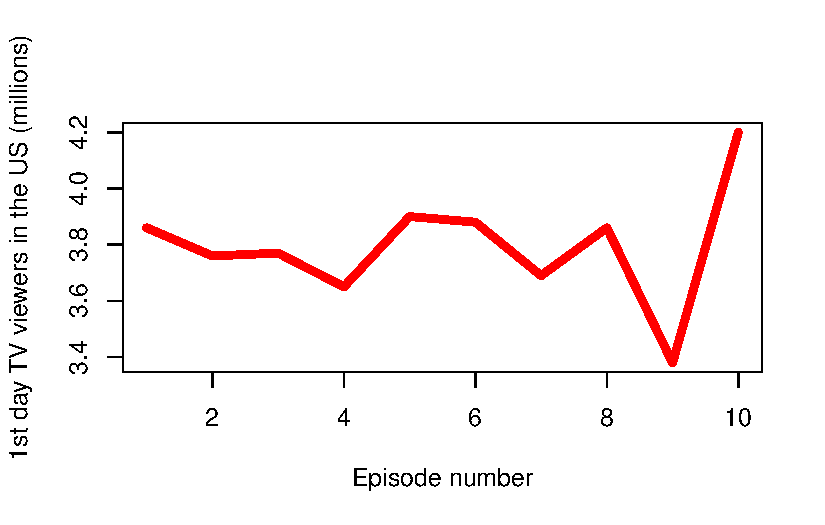
\includegraphics{Assignment_files/figure-pdf/viewers_plot-1.pdf}

\begin{center}\rule{0.5\linewidth}{0.5pt}\end{center}

Finally, the episodes with the above-average viewership were:

\begin{longtable}[]{@{}lcc@{}}
\toprule()
No.~in season & Title & Directed by \\
\midrule()
\endhead
5 & ``The Wolf and the Lion'' & Brian Kirk \\
8 & ``The Pointy End'' & Daniel Minahan \\
9 & ``Baelor'' & Alan Taylor \\
10 & ``Fire and Blood'' & Alan Taylor \\
\bottomrule()
\end{longtable}

\begin{center}\rule{0.5\linewidth}{0.5pt}\end{center}

\#Generating Reports:

\#\texttt{\{r\}\ \#quarto\_render("Assignment.qmd",\ output\_file\ =\ paste0("Report-.html"))\ \#}



\end{document}
